% **************************************************************
% Hi! Edit this file for your presentation!
% **************************************************************

% ==================///==================///==================///
% ==================/// LATEX'S STUFF
% ==================///==================///==================///

\documentclass{beamer}
\usepackage{amsfonts,amsmath,oldgerm}
\usepackage{graphics,graphicx}
\usepackage{mdframed} 
\usetheme{_statale}
\usefonttheme[onlymath]{serif}

\newcommand{\testcolor}[1]{\colorbox{#1}{\textcolor{#1}{test}}~\texttt{#1}}
\newcommand{\hrefcol}[2]{\textcolor{cyan}{\href{#1}{#2}}}
\titlebackground*{assets/background}

% ==================///==================///==================///
% ==================/// SPLASH PAGE
% ==================///==================///==================///

\title{Verifiche di compliance in ambienti Cloud}
\subtitle{Presentazione dell'elaborato finale}
\course{Laurea Triennale in Sicurezza dei Sistemi e delle Reti Informatiche}
\author{\href{mailto:niccolo.volonte@studenti.unimi.it}{Niccolò Volontè}}
\IDnumber{20642A}

% ==================///==================///==================///
% ==================///  START PRESENTATION
% ==================///==================///==================///

\begin{document}
\maketitle

\footlinecolor{maincolor}


% ==================///==================///==================///
% ==================/// BODY'S PRESENTATION
% ==================///==================///==================///

\begin{frame}{Introduzione e contesto}
    \framesubtitle{Cloud Computing e Compliance}
    \begin{itemize}
        \item Evoluzione del Cloud Computing
        \item Distinzione \emph{IaaS}, \emph{PaaS} e \emph{SaaS}
        \item Amazon Web Services (\emph{AWS}) 
        \item Compliance come sfida
    \end{itemize}
\end{frame}

\begin{frame}{Obiettivi del lavoro}
    \framesubtitle{Suite di sonde}
    \begin{itemize}
        \item Sviluppo di sonde che verificano la compliance
        \item Integrazione con la piattaforma MoonCloud
        \item Adeguamento a standard di sicurezza
        \item Automatizzazione della verifica
    \end{itemize}
\end{frame}

\begin{frame}{La compliance nel cloud}
    \framesubtitle{Significato e importanza}
    \begin{itemize}
        \item Definizione di compliance
        \item Rilevanza per la sicurezza informatica
        \item Sfide specifiche del cloud
    \end{itemize}
\end{frame}

\begin{frame}{Standard di riferimento}
    \framesubtitle{Enti, direttive e normative}
    \begin{columns}
    \begin{column}{0.6\textwidth}
        \begin{itemize}
            \item Center for Internet Security (\emph{CIS}) -
                \hrefcol{https://www.cisecurity.org/}{CIS AWS Foundations Benchmark}
            \item National Institute of Standards and Technology (\emph{NIST}) - 
                \hrefcol{https://www.nist.gov/}{NIST SP 800-53}
        \end{itemize}
    \end{column}
    \begin{column}{0.4\textwidth}
    
\includegraphics[width=\textwidth]{assets/cisnist.png}
    \end{column}
    \end{columns}
\end{frame}

\begin{frame}{Standard di riferimento}
    \framesubtitle{Esempio di controllo}
    \begin{mdframed}[backgroundcolor=statalegrey]
    \textbf{1.4 Ensure MFA is enabled for the 'root' user account (Automated)}
    \begin{itemize}
        \item \textbf{Profile Applicability:} Level 1
        \item \textbf{Description:} The 'root' user account is the most privileged user in an AWS account. Multi-factor Authentication (MFA) adds an extra layer of protection on top of a username and password. With MFA enabled, when a user signs in to an AWS website, they will be prompted for their username and password as well as for an authentication code from their AWS MFA device.
        \item \textbf{Rationale:} Enabling MFA provides increased security for console access as it requires the authenticating principal to possess a device that emits a time-sensitive key and have knowledge of a credential.
    \end{itemize} 
\end{mdframed}
\end{frame}

\begin{frame}{Tecnologie utilizzate}
    \framesubtitle{Linguaggi e strumenti}
    \begin{columns}
        \begin{column}{0.4\textwidth}
            \begin{itemize}
                \item \emph{Python} come linguaggio di programmazione
                \item \texttt{Boto3} per l'interazione con AWS
                \item \emph{MoonCloud} come piattaforma di integrazione
            \end{itemize}
        \end{column}
        \begin{column}{0.6\textwidth}
            \begin{colorblock}[black]{statalegrey}{Esempio di utilizzo di Boto3}
                \texttt{\textcolor{maincolor}{import} boto3}\\
                \texttt{client = boto3.\textcolor{maincolor}{client}(}\\
                \texttt{    \textcolor{statalegreen}{'sqs'},}\\
                \texttt{    region\_name=\textcolor{statalegreen}{'eu-central-1'},}\\
                \texttt{    aws\_access\_key\_id=\textcolor{statalegreen}{'YOUR\_ACCESS\_KEY'},}\\
                \texttt{    aws\_secret\_access\_key=\textcolor{statalegreen}{'YOUR\_SECRET\_KEY'}}\\
                \texttt{)}\\
                \texttt{response = client.\textcolor{maincolor}{list\_queues}()}\\
            \end{colorblock}
        \end{column}
    \end{columns}
\end{frame}

\begin{frame}{MoonCloud}
    \framesubtitle{Piattaforma, funzionalità e architettura}
    \begin{columns}
        \begin{column}{0.7\textwidth}
            \begin{itemize}
                \item Esegue sonde di assurance su infrastrutture ICT
                \item Architettura basata su immagini Docker e CI/CD
                \item Dashboard per la gestione dei target, credenziali e risultati
                \item Modello a stati finiti: \textit{forward}, \textit{rollback}
            \end{itemize}
        \end{column}
        \begin{column}{0.3\textwidth}
            
\includegraphics[width=\textwidth]{assets/mooncloud.png}
        \end{column}
    \end{columns}
\end{frame}

\begin{frame}{Struttura di una sonda}
    \framesubtitle{Componenti per la creazione}
    \begin{columns}
        \begin{column}{0.6\textwidth}
            \begin{itemize}
                \item Codice Python all'interno del file \texttt{probe.py}
                \item \texttt{schema.json} e \texttt{test.json} per input validato
                \item \texttt{Dockerfile}, \texttt{.gitlab-ci.yml} per la pipeline
                \item Struttura con \texttt{atoms} eseguiti in sequenza
                \item Output \emph{strutturato}
            \end{itemize}
        \end{column}
        \begin{column}{0.4\textwidth}
            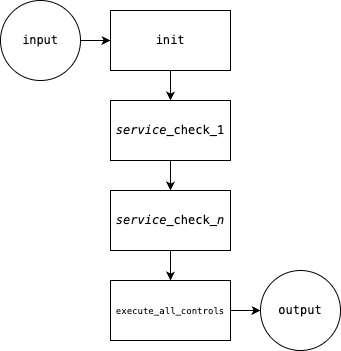
\includegraphics[width=\textwidth]{assets/flow.drawio.png}
        \end{column}
    \end{columns}
\end{frame}

\begin{frame}{Esempio di sonda}
    \framesubtitle{Sonda \texttt{aws\_sqs}}
    \begin{columns}
        \begin{column}{0.4\textwidth}
            \begin{itemize}
                \item Controlli relativi a crittografia, tagging, policy pubbliche
                \item Basata su controlli di AWS Security Hub
                \item Esempio di scansione multiregione
                \item Integra parametri personalizzati via dashboard
            \end{itemize}
        \end{column}
        \begin{column}{0.6\textwidth}
            \begin{colorblock}[black]{statalegrey}{Implementazione multiregione}
                \texttt{\textcolor{maincolor}{self}.clients = \string{\string}}\\
                \texttt{\textcolor{maincolor}{for} idx, region in \textcolor{maincolor}{enumerate}(specific\_regions, start=1):}\\
                    \texttt{    \textcolor{maincolor}{self}.clients[\textcolor{statalegreen}{f'client\_\string{idx\string}'}] = \textcolor{maincolor}{boto3}.client(}\\
                    \texttt{    \textcolor{statalegreen}{'sqs'},}\\
                    \texttt{    aws\_access\_key\_id=\textcolor{statalegreen}{'YOUR\_ACCESS\_KEY'},}\\
                    \texttt{    aws\_secret\_access\_key=\textcolor{statalegreen}{'YOUR\_SECRET\_KEY'}}\\
                    \texttt{    region\_name=\textcolor{statalegreen}{'eu-central-1'},}\\
                    \texttt{)}\\
            \end{colorblock}
        \end{column}
    \end{columns}
\end{frame}

\begin{frame}{\texttt{aws\_vulnerability}}
    \framesubtitle{Sonda per la gestione CVE}
    \begin{columns}
        \begin{column}{0.4\textwidth}
            \begin{itemize}
            \item Sonda custom che elenca CVE trovate da AWS Inspector
            \item Analisi di Elastic Container Registry (\emph{ECR}), 
                Elastic Compute Cloud (\emph{EC2}) e \emph{Lambda} functions
            \item Supporta una visione dinamica del rischio
        \end{itemize}
        \end{column}
        \begin{column}{0.6\textwidth}
            
\includegraphics[width=0.7\textwidth]{assets/mooncloud.png}
        \end{column}
    \end{columns}
\end{frame}

\begin{frame}{Esecuzione e integrazione}
    \framesubtitle{Gestione I/O e deploy}
    \begin{itemize}
        \item Input via JSON schema con validazione
        \item Gestione sicura delle credenziali
        \item Pipeline CI/CD su GitLab per ogni sonda
        \item Integrazione tramite backend di MoonCloud
    \end{itemize}
\end{frame}

\begin{frame}{Risultati ottenuti}
    \framesubtitle{Visualizzazione sulla dashboard}
    \begin{itemize}
        \item Controlli strutturati in blocchi
        \item Risultato numerico e descrittivo
        \item Sommario con percentuale di conformità
        \item Log dettagliato con eccezioni gestite
    \end{itemize}
\end{frame}

\begin{frame}{Competenze acquisite}
    \framesubtitle{Strumenti, metodologie e conoscenze}
    \begin{itemize}
        \item Tecnologie: Python, AWS, Docker, GitLab CI/CD
        \item Sviluppo modulare e orientato alla sicurezza
        \item Analisi di documentazione tecnica
        \item Esperienza in un progetto reale su una piattaforma in uso
    \end{itemize}
\end{frame}

\begin{frame}{Conclusione e sviluppi futuri}
    \framesubtitle{Riflessioni e prospettive}
    \begin{itemize}
        \item Sviluppo di 13 sonde operative
        \item Contributo concreto all'evoluzione di MoonCloud
        \vspace{0.5cm}
        \item Implementazione multiregione
        \item Estensione a nuovi benchmark e cloud provider
    \end{itemize}
\end{frame}


% ==================///==================///==================///
% ==================/// END PRESENTATION
% ==================///==================///==================///

\backmatter
\end{document}